\chapter{Introduction}

The ecoMOD project is focused on creating sustainable, prefabricated housing units in partnership with local affordable housing organizations. These units are sustainable in that are environmentally responsive, with reduced energy, water, and maintenance costs compared to traditional housing stock. ecoMOD housing is aggressively affordable without cutting corners in construction, and strives to utilize the latest best practices in green, low-impact building and construction for a total cost of ownership that is markedly less than average. As a result, ecoOMOD housing has received numerous awards and accolades in the trade space\cite{Lau2013}.

\begin{figure}
\centering
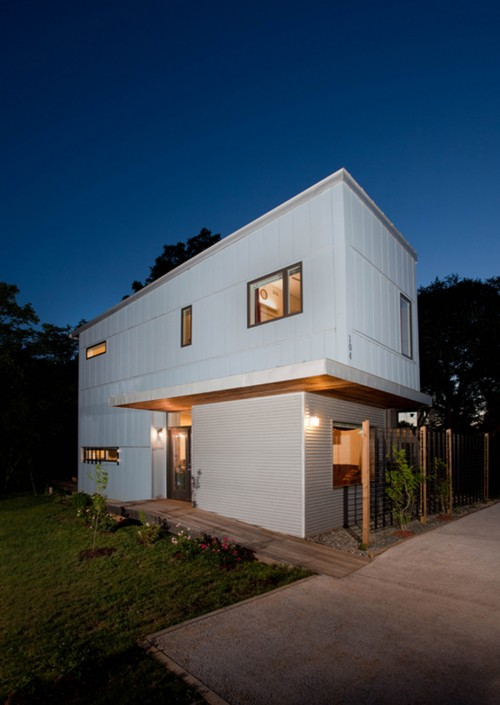
\includegraphics[width=0.3\linewidth]{./images/SFSmith_110602_8113-copy-500x705}
\caption{ecoMOD 4 in the evening\cite{Smith2011}}
\label{fig:SFSmith_110602_8113-copy-500x705}
\end{figure}

Historically, all ecoMOD housing has been extensively monitored and networked for reasons of evaluating building performance. These sensors monitor important information such as ambient temperature, humidity levels, air quality, and electricity use. This thesis is an extension of monitoring work that has been done continuously since the inception of the project, while introducing the foundations for future work in enabling environmental control. 

Existing commercial monitoring solutions usually suffer the following problem: either they are excessively costly to install in the field, or are unreliable and difficult to integrate into existing data retrieval schemes. The ecoMOD project is no stranger to sensor deployments, having previously successfully opted to use expensive commercial solutions from vendors such as National Instruments or Onset Computers. Despite the cost, systems like the ones from National Instruments are being deployed year-after-year in many different buildings. They have seen extensive use in the commercial building industry due to the greater amount of capital and land involved. This demonstrates the clear value proposition of environmental monitoring systems. If these systems could be made cheaper, more accurate, and easier to use, homeowners and renters could objectively assess and audit their building performance metrics.

The embedded systems developed in this thesis leverage current standards/software and wireless networking to create easy-to-use, Internet ready devices that can present data seamlessly and securely over the web via a representational state transfer (REST)\cite{fielding2002principled} interface. These sensors can passively collect data while consuming very little power by remaining in sleep mode for the majority of their operation, with electronics that maintain a total bill of materials  cost of less than \$30 for boards made in single quantities. This level of performance is difficult to achieve with electronics in this price range, as usually more expensive micro-controllers running full real-time operating systems are needed. In addition, exposing the sensor data via HTTP means that no embedded programming knowledge is needed to collect data from new sensors - only basic familiarity with web services programming, and knowing how to flash a firmware image.

\section{Related Literature}

In general, existing sensor network deployments use incompatible physical and application layer communication interfaces. At the physical layer, the most popular of these are IEEE 802.15.4, Bluetooth low-energy, and IEEE 802.11. At the application layer, Zigbee, Z-Wave, WirelessHART, and CoAP all enjoy significant marketshare. While there has been a push from industry players towards standardization of application and physical layer protocols, the market remains fragmented and many vendors lock customers in with proprietary and incompatible interfaces (APIs).

There are a many reasons for this. In general, most wireless sensor data must be transported to a server or data repository via the Internet anyway. Therefore, having the sensor nodes exist natively on the Internet simplifies the data transmission process, and allows greater interoperability between nodes who no longer need protocol bridges. The use of IP also allows the use of existing, mature tools for managing, provisioning, configuring, and debugging IP networks.  \todo{cite IPv6 over low power wireless personal networks, RFC 4919 IETF Aug 2007}

For a great deal of time, Internet Protocol (IP) was not used because it was considered inappropriate for use in distributed wireless sensor networks. Traditional mobile WiFi chips were targeted at laptops and cell-phones, which could be recharged on a daily or hourly basis. In addition, the protocol required too many computing resources as a proportion of microcontroller capability, especially at WiFi's higher data rates and encryption complexities. However, the problem has been solved from two sides. First, the steady advance of Moore's Law has brought down the cost in power and money of embedding computing capability. Second, the IETF has defined several reduced-functionality subsets of IP that can be implemented on smaller computers. These standards include IEEE 802.15.4, Routing over Low-Powered Lossy Networks (ROLL), and Constrained Application Protocol (CoAP). 

The device designed in this thesis utilizes a full 802.11 Internet stack along with an open hypertext interface. The adoption of IP for wireless sensor networks will speed their deployment and adoption. Communication compatibility between disparate devices will enable more competition between manufacturers, lower costs, and facilitate the creation of new services which span multiple sensor deployments. It will also allow the easy use of well-known Web technologies for aggregating and displaying sensor information.

\section{Related Devices}

\begin{figure}[h]
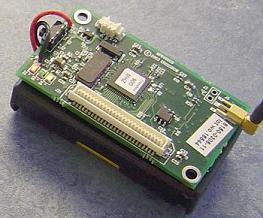
\includegraphics{images/mica2mote}
\caption{Mica2 Sensor Mote\cite{mica2mote_img}}
\label{mica2}
\end{figure}

In wireless sensor network (WSN) research, a sensor node is popularly known as a "mote", which comes from the idea that future sensor nodes will be as ubiquitous as dust motes in an Internet cloud of devices. These existing devices have been used for many years to investigate new networking techniques and to collect data for environmental monitoring. As a result, the explored design space is similar to what is designed in this thesis. 

There are many commercially available motes. Interest in distributed sensing has only increased with the ongoing media coverage of the possibilities of the "Internet of Things", which is the idea that all future electronic devices will be seamlessly interconnected via the Internet due to rapidly declining costs in wireless technology. 

Typical mote characteristics are described in Table \ref{mote_characteristics}. Generally, they include several default sensors, a low-power transceiver, an 8-bit microcontroller, and tens of kilobytes of code data and storage. As development boards they have many pins broken out for easy expandability. While bare-metal programming of these devices is popular, two operating systems exist for these platforms, where new networking and application layer protocols are tested and researched. These are Berkeley's TinyOS, and the Swedish Institute of Computer Science's (SICS) ContikiOS.

\begin{table}[h]
\begin{tabular}{@{}lllll@{}}
\toprule
Processor & Platform Name & Speed (MHz) & Ram (Kb) & Transceiver \\ \midrule
TI MSP430 & TelosB & 8 & 10 & TI CC2420 \\
Atmel ATMega 128 & MICA & 8 & 4 & Atmel RF230 \\
MC1322x & Econotag & 26 & 128 & MC1322x \\
Atmel ATMega 128 & Waspmote & 14 & 8 & Varies \\ \bottomrule
\end{tabular}
\caption{Typical Mote Characteristics}
\label{mote_characteristics}
\end{table}

\section{Contributions}

This thesis describes a method for designing a development platform that allows for further research and monitoring into building performance envelopes. Power consumption is analyzed, and various methods for extending battery lifetime are explored. Chapter 1 explores the hardware design choices. Chapter 2 does a similar exploration of the firmware load. Chapter 3 presents a short overview of various energy trade-offs, followed by Chapter 4, which contains a conclusion and a summary of further work.